% !TEX root = ../../my-thesis.tex
%
\graphicspath{{./content/part_II/figures/}}

\chapter*{Introduction}

This introduction is greatly inspired from Arnulf Jentzen lecture notes "On Deep Artificial Neural Networks and Machine Learning for PDEs" (\textsc{Deep\_Neural\_Network\_028.pdf}) and "Numerical Analysis of Stochastic Ordinary Differential Equations" (\textsc{NASODE\_Lecture\_Notes.pdf}).

% some guys that have had problems with curse of dimensionality in Finance: https://scicomp.stackexchange.com/questions/8465/are-there-finite-element-software-who-handles-more-than-five-dimensions

\section*{Towards a Deep Learning-based approximation for PDEs}

\subsection*{Curse of dimensionality}
Standard approximation methods for nonlinear PDEs, such as finite difference approximation methods, finite element approximation methods, spectral Galerkin approximation methods, sparse grid approximation methods, and standard nested Monte Carlo approximation methods, suffer from the so-called curse of dimensionality in the sense that the number of computational operations of the employed approximation scheme grows exponentially in the PDE dimension $d \in N $or in the reciprocal $1/\epsilon$ of the prescribed approximation accuracy $\epsilon \in (0, \infty)$ and it is a very challenging problem to design and analyze approximation methods for nonlinear PDEs which overcome the curse of dimensionality in the sense that the number of computational operations of the proposed approximation algorithm grows at most polynomially in the PDE dimension $d \in N$ and in the reciprocal $1/\epsilon$ of the prescribed approximation accuracy $\epsilon \in (0, \infty)$. \cite{Beck2020}

\subsubsection*{A concrete example for the finite difference scheme}
For an ODE which solution is $u \colon [0,T] \to \R$, one needs to discretize the interval $[0,T]$ in $N_t$ time steps to find variables $u_1, \dots, u_{N_t}$ approximating $u(t_1), \dots, u(t_{N_t})$. Such variables can be found by solving a system of linear equations, in the case of an explicit scheme. For a PDE which solution is $u \colon [0,T] \times D \to \R$, $D\subseteq \R^d$ one needs to discretize the time space and the domain $D$. Assuming that dimension $i$ of $D$ is discretized in $N_i$, then one needs to write a linear system of equations with $N_t N_1 \dots N_d$ variables corresponding to $u(t_1, x_1^{(1)}, \dots, x_d^{(1)}), \dots, u(t_{N_t}, x_1^{(N_1)}, \dots, x_d^{(N_d)})$. Assuming that $N_t, N_1, \dots, N_d > N$, this means the number of variables to solve for is  greater than $N^{d+1}$. This means that the computational cost grows exponentially in the number of the dimension of the PDE.

\begin{figure}
    \center
    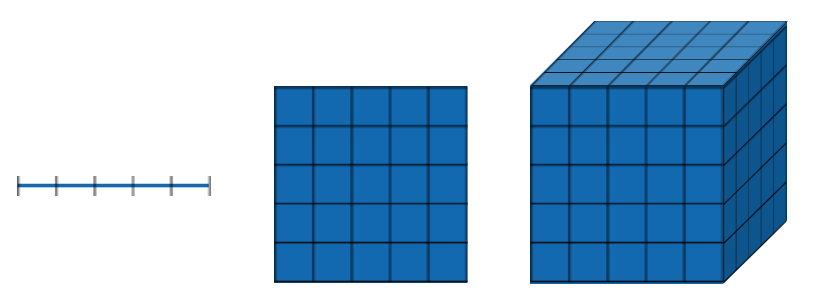
\includegraphics{curse_dim_finite_diff.png}
    \caption{Illustration of the curse of dimensionality with a finite difference scheme}
\end{figure}

\subsection*{Diffusion approximation}
\begin{proposition}[Diffusion approximation]
    Let $d \in \N$, 
    $t \in (0, \infty)$, 
    $\sigma \in \R$,
    $a \in \R$,
    $b \in (0, \infty)$, 
    let 
    $\phi \colon \R^d \to \R$ 
    be a function,
    let 
    $u \in C^{1,2}([0,T] \times \R^d, \R)$ 
    be a function with at most polynomially growing partial derivatives which satisfies for every 
    $t\in [0,T]$,
    $x \in \R^d$ 
    that
    $u(0, x) = \phi(x)$ 
    and
    \begin{equation}
        \partial_t u(t, x) = \tfrac{1}{2} \sigma^2 \Delta_x u(t,x),
    \end{equation}
    let $(\omega, \F, \P)$ be a proability space, and let $\W \colon \Omega\to\R^d$ be a standard normal random variable.
    Then
    \begin{enumerate}[label=(\roman*)]
        \item it holds that the function $\phi \colon \R^d \to \R$ is twice continuously differentiable with at most polynomially growing derivatives and 
        \item it holds for every $x \in \R^d$ that $u(T, x) = \E\left[ \phi(\sigma \W \sqrt{T} + x)\right]$
    \end{enumerate} 
\end{proposition}

Note that here above we think of $\sigma \W \sqrt{T}$ as $\sigma B_T$ where $B_T$ is a standard Brownian motion.

\begin{figure}
    \center
    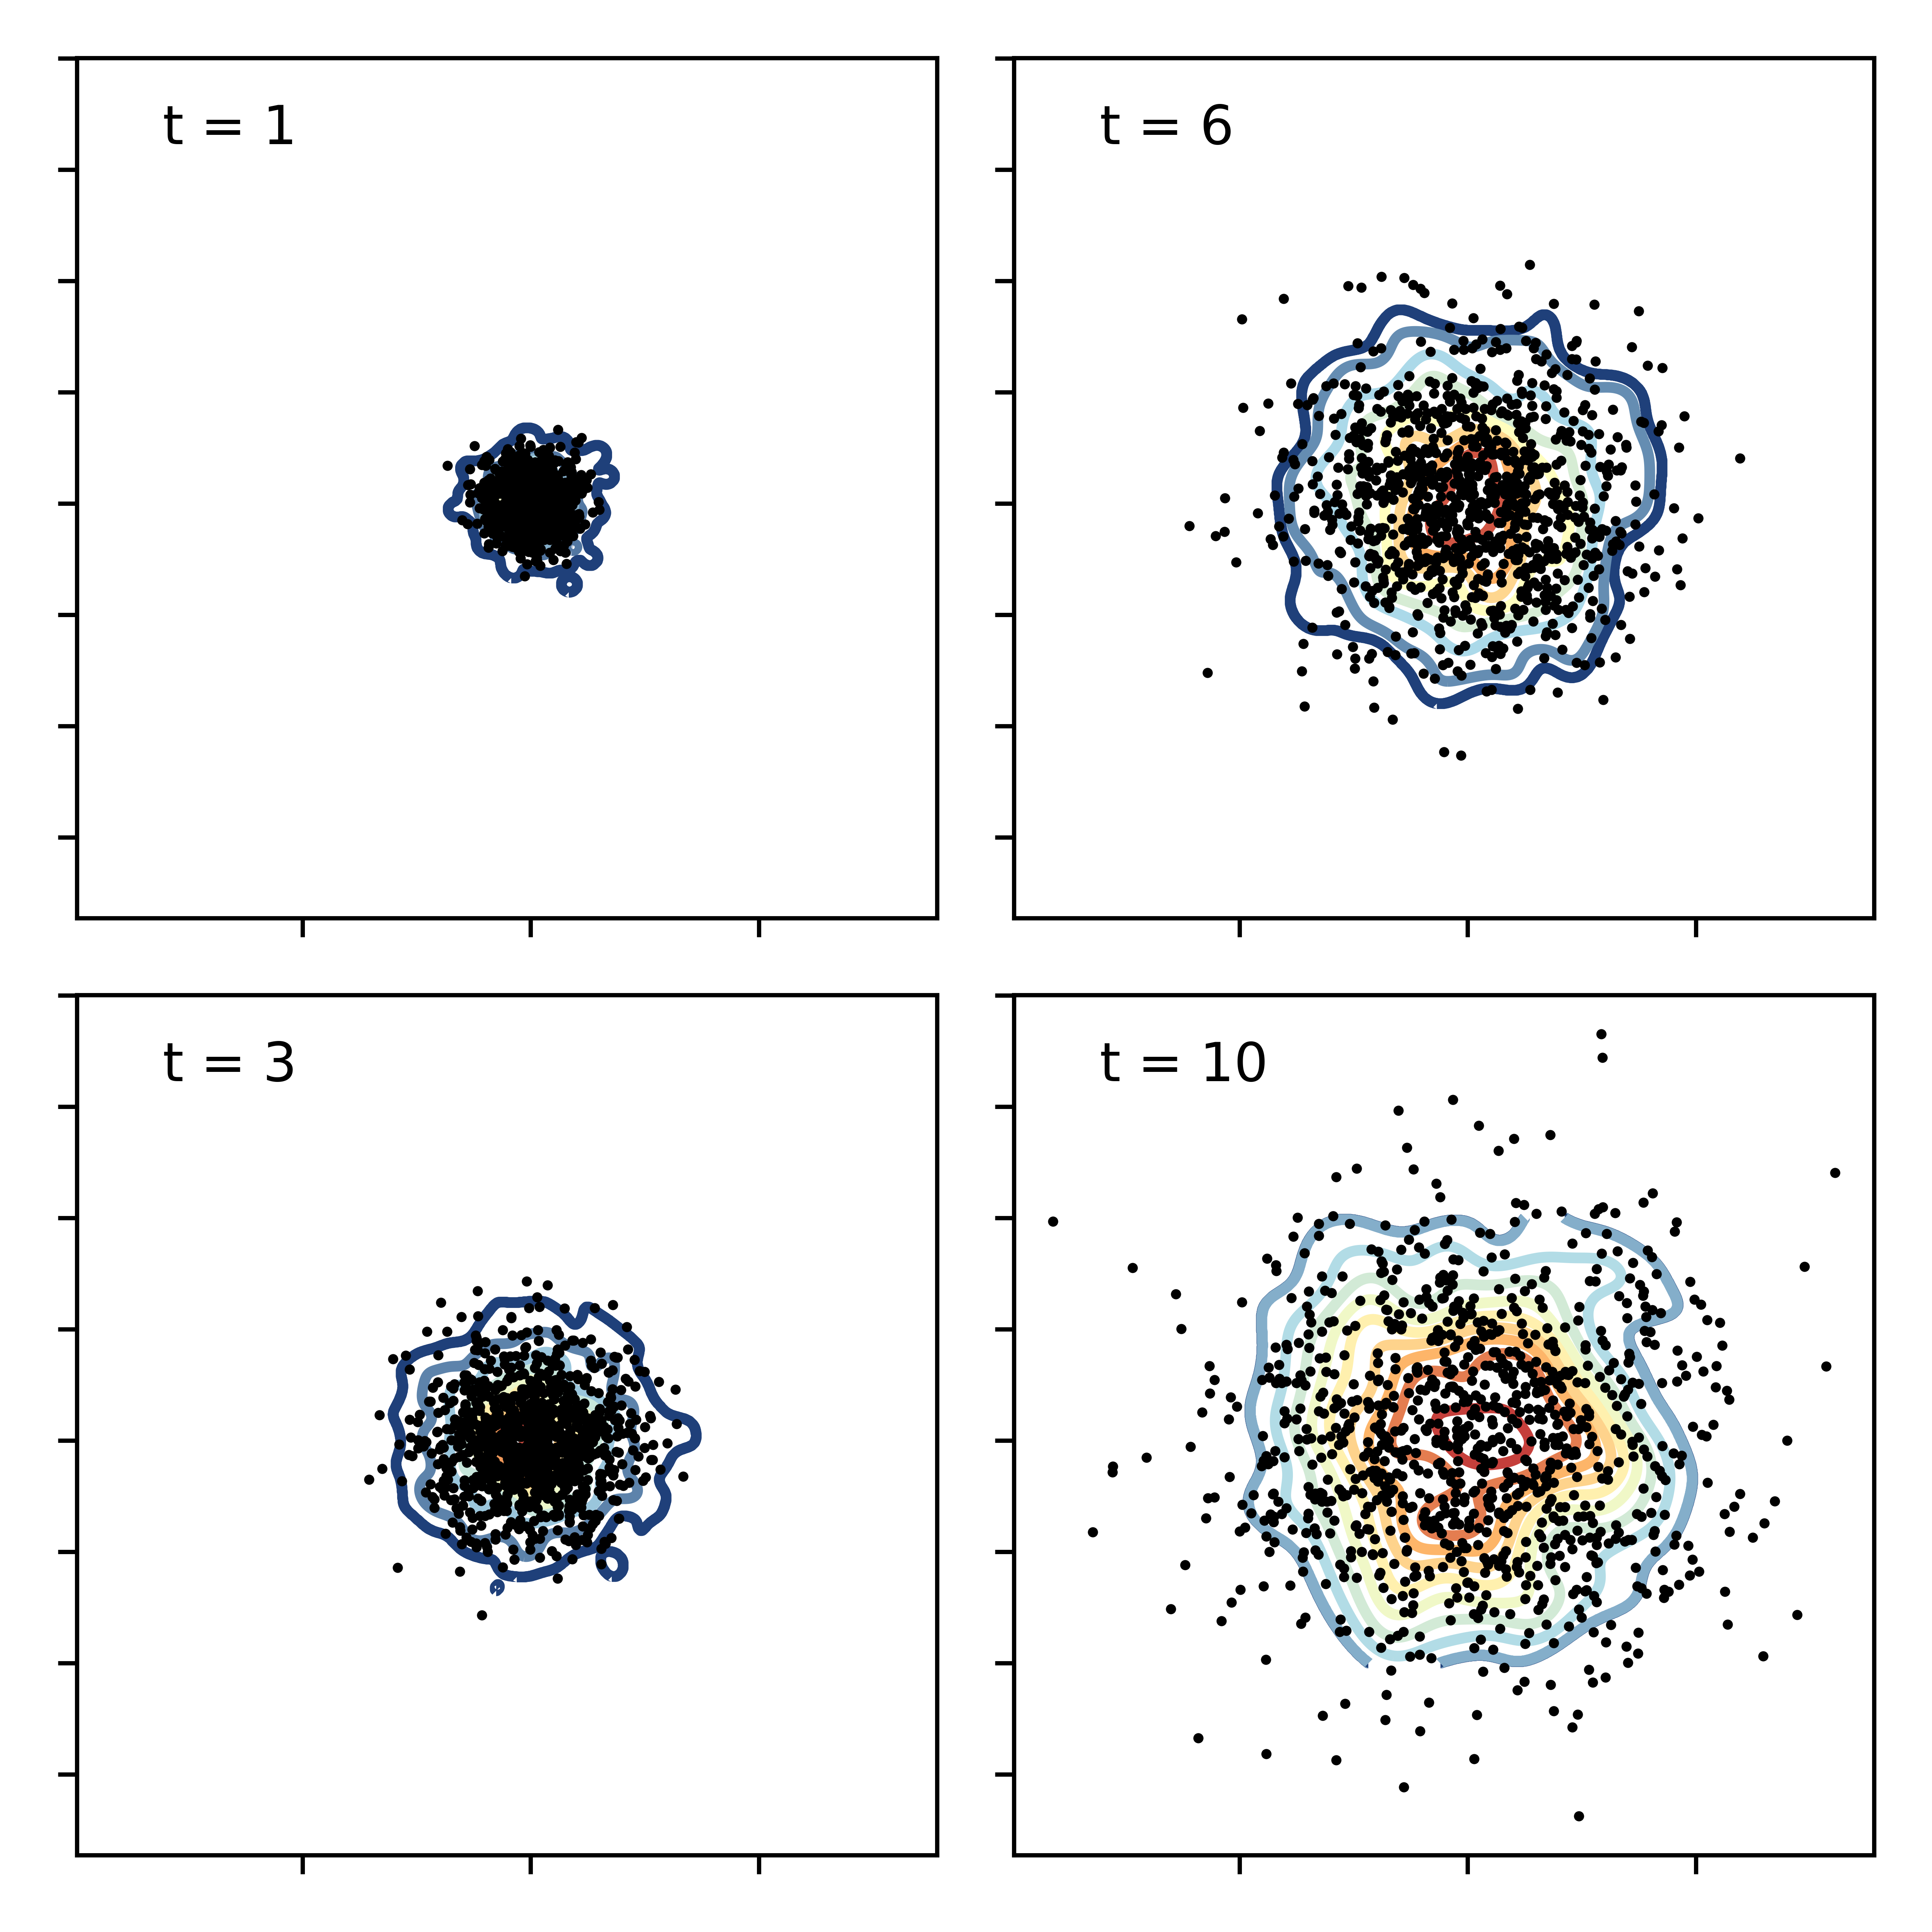
\includegraphics[width=0.5\textwidth]{brownian_motion_diffusion.png}
    \caption{Brownian motion diffusion. Contour line represent estimated particle density.}
\end{figure}

\subsection*{Monte Carlo integration}
Here we show that the above expectation can be approximated by a Monte Carlo averaging
\begin{equation}
    \E\left[ \phi(\sigma \W \sqrt{T} + x)\right] \approx \frac{1}{M} \sum_{m=1}^M \left[ \phi(\sigma \W^{(m)} \sqrt{T} + x) \right]
\end{equation}
and that the approximation error is proportional to $\sqrt{N}$ so that a Monte Carlo approach combined with the diffusion approximation overcomes the curse of dimensionality.

\subsection*{Deep Learning-based approximation}

A genuine idea to approximate $u$ on the whole interval $[a,b] \subseteq \R^d$ is to introduce a function approximator 
%  Victor: this is to change
$\NN_\theta(x) = \sigma_l (W_l (\dots (W_2 \sigma_1 (W_1 x + b_1) + b_2) \dots ) + b_l$
where 
$W_i$, $b_i$ 
are respectively the weights and biases at level $i$, and $\theta = \{W_1, \dots, W_l, b_1, \dots, b_l\}$ denotes the ensemble of parameters. Note that in the following we adopt an other perspective on neural networks, dealing with layers and neurons instead of matrix multiplications.

Cost function 
\begin{equation}
    \mathcal{L}_{\theta} = \frac{1}{M} \sum_{m=1}^M \left[ \NN_\theta^{(m)}(\xi^{(m)}) - \phi \left( \sigma B_T^{(m)} + \xi^{(m)}\right) \right]^2
\end{equation}

\subsection*{Prerequisites}
This leads to the 
\begin{theorem}[Non-linear Feynman Kac for initial value problems]
Consider the PDE
\begin{equation}
    \partial_t u(t,x) = \mu(t, x) \nabla_x u(t,x) + \frac{1}{2} \sigma^2(t, x) \Delta_x u(t,x) + f(x, u(t,x))
\end{equation}
with initial conditions $u(0, x) = g(x)$, where $u \colon \R^d \to \R$. 
Then
\begin{equation}
    u(t, x) = \int_0^t \mathbb{E} \left[ f(X^x_{t - s}, u(T-s, X^x_{t - s}))ds \right] + \mathbb{E} \left[ u(0, X^x_t) \right] \tag{3}
\end{equation}
with 
\begin{equation}
    X_t^x = \int_0^t \mu(X_s^x)ds + \int_0^t\sigma(X_s^x)dB_s + x.
\end{equation}

\end{theorem}

State contribution

\section*{Parameter inference for Differential Equations}

Reverse engineering

Approximate Bayesian Computation in Evolution and Ecology : \cite{Beaumont2010}

Parametric estimation applied to predict community stability: \cite{Cenci2019}

adjoint for solver 

State contribution
